\documentclass[11pt,a4paper]{article}

\usepackage[T1]{fontenc}
\usepackage[utf8]{inputenc}
\usepackage[margin=1in]{geometry}
\usepackage{booktabs}
\usepackage{graphicx}
\usepackage{amsmath}
\usepackage{amssymb}
\usepackage{microtype}
\usepackage[hidelinks]{hyperref}
\usepackage{natbib}
\usepackage{caption}

\bibliographystyle{plainnat}

% Confidence intervals are set small and grey-free so they read as an
% annotation on the mean and do not compete with it for attention.
\newcommand{\ci}[2]{{\footnotesize $[#1,\,#2]$}}
\newcommand{\yes}{yes}
\newcommand{\no}{no}

% Every number quoted in the prose comes from here, generated from results/*.csv
% by scripts/make_paper_tables.py.
% Generated by scripts/make_paper_tables.py. Do not edit by hand.
% Every number quoted in the prose is defined here, straight from
% results/*.csv, so the text cannot drift from the experiments.
\newcommand{\BaseRate}{34.4}
\newcommand{\BestComposite}{HST, periodic}
\newcommand{\BestCompositeLosses}{4}
\newcommand{\BestCompositeVal}{0.606}
\newcommand{\BestPA}{HST, online}
\newcommand{\BestPAVal}{0.794}
\newcommand{\BestPoint}{iForest, drift}
\newcommand{\BestPointVal}{0.539}
\newcommand{\BestRange}{iForest, periodic}
\newcommand{\BestRangeVal}{0.198}
\newcommand{\BestUcrComposite}{iForest, never}
\newcommand{\BestUcrCompositeVal}{0.033}
\newcommand{\BestUcrFound}{0.50}
\newcommand{\BestUcrFoundPolicy}{never rebuild}
\newcommand{\BestUcrName}{LOF, never}
\newcommand{\BestUcrPoint}{LOF, never}
\newcommand{\BestUcrPolicy}{never rebuild}
\newcommand{\BestUcrTopOne}{MCD, never}
\newcommand{\BestUcrTopOneVal}{0.12}
\newcommand{\FastestModel}{OC-SVM, never}
\newcommand{\FastestRows}{129,212}
\newcommand{\FlagAll}{0.512}
\newcommand{\FlagAllPA}{0.512}
\newcommand{\FlagAllRange}{0.045}
\newcommand{\MaxRankJump}{6}
\newcommand{\MeanUcrTopOne}{0.06}
\newcommand{\MoverComposite}{0.576}
\newcommand{\MoverCompositeRank}{2nd}
\newcommand{\MoverName}{HST, drift}
\newcommand{\MoverPoint}{0.477}
\newcommand{\MoverPointRank}{8th}
\newcommand{\NBeatComposite}{10}
\newcommand{\NBeatPA}{10}
\newcommand{\NBeatPoint}{7}
\newcommand{\NBeatRange}{3}
\newcommand{\NComparisons}{48}
\newcommand{\NDistinctWinners}{4}
\newcommand{\NNabBeatsComposite}{6}
\newcommand{\NNabBeatsPoint}{3}
\newcommand{\NNabDistinctWinners}{5}
\newcommand{\NNabSeries}{6}
\newcommand{\NRankChanges}{10}
\newcommand{\NRecordings}{15}
\newcommand{\NRows}{17,160}
\newcommand{\NSeedComparisons}{8}
\newcommand{\NSeedSignificant}{7}
\newcommand{\NSeeds}{10}
\newcommand{\NSignificant}{36}
\newcommand{\NStrategies}{10}
\newcommand{\NUcrAdaptive}{4}
\newcommand{\NUcrAdaptiveAboveBest}{0}
\newcommand{\NUcrBeatComposite}{8}
\newcommand{\NUcrBeatPoint}{1}
\newcommand{\NUcrSeries}{8}
\newcommand{\NabEventRecallMin}{0.00}
\newcommand{\SkabEventRecallMin}{1.00}
\newcommand{\SlowestModel}{iForest, drift}
\newcommand{\SlowestRows}{844}
\newcommand{\SpeedRatio}{153}
\newcommand{\SpeedSource}{a quiet run}
\newcommand{\SteadiestLosses}{0}
\newcommand{\SteadiestName}{iForest, periodic}
\newcommand{\TopOneAgreesWithComposite}{no}
\newcommand{\UcrBaseRate}{1.05}
\newcommand{\UcrFlagAll}{0.020}
\newcommand{\UcrRecallSpread}{0.25}
\newcommand{\UcrRows}{8,392}
\newcommand{\WorstComposite}{OC-SVM, never}
\newcommand{\WorstCompositeVal}{0.513}
\newcommand{\WorstPA}{OC-SVM, never}
\newcommand{\WorstPAVal}{0.513}
\newcommand{\WorstPoint}{HST, online}
\newcommand{\WorstPointVal}{0.314}
\newcommand{\WorstRange}{LOF, never}
\newcommand{\WorstRangeVal}{0.001}
\newcommand{\WorstUcrFound}{0.25}
\newcommand{\WorstUcrName}{OC-SVM, never}
\newcommand{\WorstUcrTopOneVal}{0.00}


\captionsetup{font=small,labelfont=bf}
\setlength{\parskip}{0pt}

\title{Scoring conventions reorder adaptation policies in\\ streaming anomaly detection}

\author{%
  Dhruvil Amit Shah\\
  {\normalsize Independent Researcher \textperiodcentered{} contactshahdhruvil@gmail.com \textperiodcentered{} ORCID 0009-0008-2988-5216}
}

\date{Preprint \textperiodcentered{} September 2026, revised November 2026\\[2pt]
\small Code and data: \url{https://github.com/DhruvilShah22/drift-aware-anomaly-detection} \textperiodcentered{} License: CC BY 4.0\\
Cite as: D. A. Shah, ``Scoring conventions reorder adaptation policies in streaming anomaly detection,'' Zenodo, 2026, doi:10.5281/zenodo.22333125.}

\begin{document}
\maketitle

\begin{abstract}
A streaming anomaly detector has to decide when to rebuild itself once its input
starts to drift. We compare four ways of handling that, keeping everything else the
same: never rebuild, keep learning all the time, rebuild on a schedule, or rebuild
when a drift detector goes off. We scored the same runs under four published
conventions and got \NDistinctWinners{} different winners. Same predictions, too.
\MoverName{} comes \MoverPointRank{} of \NStrategies{} under point-wise F1 and
\MoverCompositeRank{} under the composite F-score. The comparison covers \NSeeds{}
seeds and the \NRecordings{} source recordings that have a fault in them, with paired
tests and Holm correction. We also pull apart two things that usually get lumped
together: the anomaly model and the adaptation policy. On this data, the best policy
is whichever one your scoring happens to favour. Every one of the \NStrategies{}
strategies changes rank between point-wise and composite scoring, and the biggest
jump is \MaxRankJump{} places. Then there's a third dataset, the UCR Anomaly Archive,
which was built to replace benchmarks its authors thought were flawed. There, none of
this matters much. No policy stands out from the rest, and by the archive's own
threshold-free test the best of the ten puts its peak score inside the labelled window
on \BestUcrTopOneVal{} of series. Code, logs and every table here come back from a
single command.
\end{abstract}

\section{Introduction}

A detector trained once on a sensor stream goes wrong in one of two directions
as the process it watches changes. If it never updates, ordinary operation
drifts away from what it learned and it flags almost everything. If it updates
continuously, it absorbs the change into its own idea of normal and goes quiet,
so a fault that arrives slowly is learned rather than reported. Both failures
are easy to build by accident and neither is visible in a single accuracy
number.

The question this raises is not whether anomalies can be detected but
\emph{when the detector should update itself}. That question has an established
shape: monitor the input, and when a change-detection test fires, rebuild. What
it does not have is an established answer, because the evidence for one policy
over another is usually a single number from a single run, scored under
whichever convention the authors preferred.

We built the comparison carefully enough to find out, and the result was not
the one we set out to report. Our own earlier version of this work, run once at
one seed and scored point-wise, concluded that a periodic rebuild schedule was
best and that the continuously-learning control was broken. Both conclusions
turned out to be properties of the scoring convention, not of the
detectors. Under event-level scoring the control catches every fault in the
stream, and the ranking of the policies rearranges.

This paper reports that finding properly. Our contributions:

\begin{enumerate}
\item \textbf{A convention-crossed comparison.} The same runs are scored under
  point-wise F1, the composite F-score of \citet{garg2021evaluation},
  range-based precision and recall \citep{tatbul2018range}, and point-adjust
  \citep{xu2018donut} with its PA\%K repair \citep{kim2022rigorous}. The
  conventions disagree about which adaptation policy is best.
\item \textbf{A factorial design.} Adaptation policy and anomaly model are
  crossed, so a difference can be attributed to one or the other. The usual
  presentation compares a static Isolation Forest against an adaptive
  Half-Space Trees model and calls the difference adaptation.
\item \textbf{Replication and paired tests.} Every result is repeated over
  \NSeeds{} seeds and over the \NRecordings{} source recordings that carry a
  fault. Comparisons are paired within a seed and within a recording,
  with Holm correction over the family of comparisons we report.
\item \textbf{Negative results stated as such.} Whether a strategy beats the
  F1 obtained by flagging every single row is itself convention-dependent:
  \NBeatPoint{} of \NStrategies{} clear it point-wise, \NBeatComposite{}
  under the composite score, and \NBeatRange{} under range-based scoring (only
  \NBeatRangeClear{} with the whole interval above the baseline). We
  report the baseline beside every result, and did not go looking for the
  convention that flatters ours.
\end{enumerate}

\section{Related work}

\paragraph{Adapting to concept drift.} \citet{gama2014survey} organise the field
into detectors that signal a change and learners that respond to one. ADWIN
\citep{bifet2007adwin} keeps a window it cuts whenever two sub-windows differ
enough in mean, which gives it a change point without a fixed window size.
KSWIN \citep{raab2020kswin} runs a Kolmogorov-Smirnov test between a reference
sample and a sliding one. The Page-Hinkley test \citep{page1954cusum} integrates
a one-sided deviation and fires when the running sum exceeds a threshold. Larger
comparisons of detectors exist \citep{barros2018largescale}, though they are
usually framed around supervised classification error, not the unlabelled
input statistic this project watches. Section~\ref{sec:monitoring} gives the
reason for watching the input at all.

\paragraph{Streaming anomaly detection.} Half-Space Trees \citep{tan2011hst}
score a point by the mass of the region it falls into, over an ensemble of
random trees with fixed feature ranges, and update in constant time per
observation. Isolation Forest \citep{liu2008iforest} isolates points by random
splits and is the usual static baseline. Local Outlier Factor
\citep{breunig2000lof}, the one-class SVM \citep{scholkopf2001ocsvm} and the
minimum covariance determinant estimator \citep{rousseeuw1999mcd} are the
classical alternatives; none supports an incremental update, so for them
adaptation can only mean a refit. More recent systems adapt by pooling models
without resetting one \citep{yoon2022arcus}. We use the simpler reset
because the object of study here is the policy, not the model.

\paragraph{How these systems are scored.} This is where the field is least
settled, and it is the part our results turn on. Point-wise F1 treats every row
independently and rewards a detector for flagging every row of a long fault,
which is not what an operator wants. \citet{xu2018donut} introduced point-adjust,
under which one flagged row inside a true segment credits the detector with the
whole segment; \citet{kim2022rigorous} showed that this inflates scores so far
that random predictions beat published models, and proposed PA\%K, which only
credits a segment when at least $K$ of it was flagged. \citet{tatbul2018range}
give a range-based precision and recall that scores existence, overlap and
fragmentation separately. \citet{garg2021evaluation} define a composite
F-score that pairs point-wise precision with event-level recall.
\citet{paparrizos2022vus} and \citet{huet2022affiliation} propose further
alternatives. \citet{wu2023flawed} argue that several widely-used benchmarks,
including the one we use as a second dataset, are flawed enough to create an
illusion of progress.

Our position is narrower than a survey of these proposals. We take four of them
as given, apply them to one set of runs, and report that they do not agree about
which adaptation policy to use. The disagreement is the result; we are not
arguing that any one of the four is correct.

\section{Setup}

\subsection{Adaptation policies}

Every policy sees the same stream, the same warm-up length and the same alarm
threshold. The only thing that differs is when, or whether, the model is
rebuilt.

\begin{description}
\item[never] The model is fitted once on the warm-up window and left alone.
\item[online] The model keeps learning from every row and is never explicitly
  rebuilt. It is a control and not a policy, and it matters: without it,
  \emph{never} and \emph{periodic} would differ in the model as well as the
  schedule.
\item[periodic] The model is rebuilt every 1{,}000 rows, whether or not
  anything has changed.
\item[drift] The model is rebuilt when a drift monitor fires on the input.
\end{description}

Rebuilding always means the same operation: re-run warm-up on the most recent
1{,}000 rows, which regenerates the model, its feature ranges and its threshold
together. Between rebuilds every policy except \emph{online} holds the model
fixed. A retraining policy that also learns continuously is not really a
retraining policy, and in an earlier version of this work it collapsed into the
control.

\subsection{Models}

Half-Space Trees is the online model. Isolation Forest, LOF, the one-class SVM
and the MCD estimator are the static ones. Crossing the models with the policies
gives the grid in Table~\ref{tab:main}; the three classical baselines appear
only under \emph{never}, since they cannot be updated incrementally.

Two implementation choices are worth stating because they are what makes the
comparison mean anything. Feature ranges are fixed at warm-up and never
rolled forward. The usual choice is a min-max scaler, but it adapts continuously and
would absorb the drift before the model ever saw it, hiding the effect being
measured. The alarm threshold is likewise a quantile of the warm-up scores, held
until the next rebuild. Half-Space Trees normalises its raw score against a
maximum that is essentially never reached, so scores sit in a narrow offset band
and an absolute threshold is meaningless.

\subsection{Drift monitoring}
\label{sec:monitoring}

The drift monitor watches the input, not the model's anomaly score. Watching the
score is self-defeating for a learning model: it accommodates the shift, its
score distribution does not move, and the detector never fires. In an earlier
run that produced zero detections on the labelled stream. The monitored signal
is the mean absolute $z$-score of the sensors, standardised against the window
the model was last built on, so it answers ``has the world moved since this
model was built''. The reference is refit on every rebuild.

Because the schedule depends only on this input statistic, it is computed in one
cheap pass and the scoring is done afterwards in blocks; a test asserts that this
gives the same flags, scores and adaptation points as the plain loop.

\subsection{Thresholds}

The alarm threshold is a quantile of the warm-up score distribution. It encodes
how often anomalies are expected, and the dataset families here differ by more
than an order of magnitude in base rate, so a single value across all of them
would not be a fair comparison but a badly calibrated detector on most. We use
$q=0.50$ on the labelled SKAB stream, which is \BaseRate\% anomalous, and
$q=0.98$ on the injected, NAB and UCR streams. Section~\ref{sec:transfer} measures
what carrying one setting to a new dataset costs.

\section{Evaluation conventions}

We score every run four ways. Let the ground truth be a set of contiguous
\emph{events} and the prediction a set of flagged rows.

\paragraph{Point-wise.} Precision, recall and F1 over rows, each scored
independently.

\paragraph{Composite.} Point-wise precision with event-level recall: an event
counts as recalled if any row inside it was flagged, while precision still pays
for every false row. This is the composite F-score of
\citet{garg2021evaluation}. We arrived at it independently before finding it in
the literature, and our test suite asserts that the two definitions agree.

\paragraph{Range-based.} The precision and recall of \citet{tatbul2018range},
with a flat positional bias and the reciprocal cardinality factor, so a true
range detected in many fragments scores below the same coverage detected in one.
We report $\alpha = 0$, pure overlap, and give $\alpha = 1$, pure existence, as a
sensitivity.

\paragraph{Point-adjust.} The convention of \citet{xu2018donut}, and PA\%K at
$K=0.2$ \citep{kim2022rigorous}. We report point-adjust to show what it does to
our ranking, and we do not rely on it. On SKAB's fault blocks, which
average about 390 rows, crediting a whole block for one flagged row is a very
large gift.

Every result is quoted against the F1 obtained by flagging every single row,
which at a base rate $b$ is $2b/(1+b)$. On the labelled stream that is
\FlagAll{}. An F1 in the low 0.5s means nothing next to it, and reporting one
without it would be misleading.

\section{Experimental design}

\subsection{Data}

\textbf{SKAB} \citep{katser2020skab} is a labelled industrial testbed with eight
sensors. Our labelled stream concatenates 16 \texttt{valve1} recordings, giving
\NRows{} scored rows at a \BaseRate\% anomaly rate; the individual recordings
are too short to warm up on and still leave stream to measure. \NRecordings{}
of the 16 contain a labelled fault and are scored separately in
Section~\ref{sec:replication}; the remaining one has none, and an F1 on it
would be zero for every strategy alike. The joins between recordings are real regime changes of unknown size,
so this stream is used for anomaly quality only and never for drift timing.

\textbf{Injected streams} are built by applying a known shift to SKAB's
anomaly-free recording in four shapes: sudden, incremental, gradual and
recurring. They contain no true anomalies by construction, which is what makes
them useful: change points are known to the row, so timing is exact, and every
flag raised is by definition a false alarm.

\textbf{NAB} \citep{lavin2015nab} is the second dataset, used to test whether a
calibration transfers. It differs from SKAB in the ways that would break one: it
is univariate where SKAB has eight sensors, and roughly 10\% anomalous where
SKAB is \BaseRate\%. We use \NNabSeries{} series long enough to warm up on.

\textbf{The UCR Anomaly Archive} \citep{wu2023flawed} is the third. Its authors
argued that NAB and benchmarks like it are flawed enough to create an illusion of
progress, and built the archive as a replacement: 250 univariate series, each with
exactly one anomaly and a clean training prefix. That is what SKAB lacks. On SKAB
every strategy catches every labelled event, so event-level recall is 1.0 for all
of them; with one short anomaly per series, the proportion found becomes a
measurement and not a constant.

The full archive at \NSeeds{} seeds is too much for one core, so we take
\NUcrSeries{} series under a rule fixed in advance
(\texttt{data\_loader.select\_ucr\_series}): at most 12{,}000 rows, a clean
prefix longer than the warm-up window, an anomaly under a tenth of the series,
and at most one series per source signal, in archive-index order. The last
condition matters because the archive's 251 files cover only 42 source signals
under varied names; without it, our first subset was mostly two signals.
\NUcrSeries{} is also where the archive divides: the next-shortest distinct
signal is 24{,}667 rows long. The selected series average \UcrRows{} rows at a
\UcrBaseRate\% anomaly rate, which puts the trivial baseline at \UcrFlagAll{}
against \FlagAll{} on SKAB.

\subsection{Replication and pairing}

Each run is repeated at \NSeeds{} seeds. A seed drives the model, the drift
detector where it samples, and the gradual injection, the only stream that draws
randomly. Runs are paired: at a given seed every strategy sees the same stream
and the same warm-up, which matters because the between-seed spread is larger
than the gap between policies.

The second unit of replication is the more informative one. Every strategy is
also scored on each of the \NRecordings{} source recordings that contain a
fault. Seeds ask whether a gap survives the randomness; recordings ask whether
it survives the data. A policy that is stable across seeds and unstable across
recordings has not been shown to work.

\subsection{Statistics}

Intervals are percentile bootstrap intervals over 10{,}000 resamples
\citep{efron1979bootstrap}. Comparisons use the Wilcoxon signed-rank test
\citep{wilcoxon1945} on the paired differences, in place of a $t$-test, because
the metrics are bounded, skewed and occasionally pinned at 0 or 1. We apply
Holm-Bonferroni correction \citep{holm1979sequential} within each stream, over
the family of comparisons the paper actually makes.

One caveat is built into the reporting. With $n$ paired samples the smallest
attainable two-sided $p$ from the exact signed-rank test is $2/2^n$, so below six
pairs no effect of any size can reach $p<0.05$. Comparisons below that threshold
are flagged as underpowered and never counted as significant, because a
non-significant verdict there is a property of $n$ and not of the data
\citep{demsar2006statistical}.

The models come from \texttt{river} \citep{montiel2021river} and
\texttt{scikit-learn} \citep{pedregosa2011sklearn}, and the full grid runs on one
laptop core in under an hour.

%% ------------------------------------------------------------------
%% RESULTS
%% ------------------------------------------------------------------
\section{Results}
\label{sec:results}

\subsection{The convention decides the ranking}
\label{sec:ranking}

Table~\ref{tab:main} scores one set of runs four ways. The predictions are
identical down the row; only the function applied to them changes.

\begin{table}[t]
\centering
\begin{tabular}{lccccc}
\toprule
 & \multicolumn{4}{c}{F1 under each convention} & \\
\cmidrule(lr){2-5}
Model, policy & Point-wise & Composite & Range & Point-adj. & Alarm rate \\
\midrule
HST, never & 0.377 \ci{0.346}{0.409} & 0.531 \ci{0.512}{0.549} & 0.008 \ci{0.008}{0.009} & 0.742 \ci{0.722}{0.761} & 0.380 \\
HST, online & 0.314 \ci{0.292}{0.334} & 0.523 \ci{0.516}{0.529} & 0.007 \ci{0.007}{0.007} & 0.794 \ci{0.777}{0.811} & 0.278 \\
HST, periodic & 0.517 \ci{0.509}{0.527} & 0.606 \ci{0.599}{0.613} & 0.045 \ci{0.029}{0.067} & 0.707 \ci{0.704}{0.710} & 0.505 \\
HST, drift & 0.477 \ci{0.471}{0.483} & 0.576 \ci{0.570}{0.581} & 0.024 \ci{0.022}{0.027} & 0.700 \ci{0.696}{0.703} & 0.496 \\
iForest, never & 0.514 \ci{0.513}{0.515} & 0.514 \ci{0.513}{0.515} & 0.026 \ci{0.006}{0.052} & 0.514 \ci{0.513}{0.515} & 0.995 \\
iForest, periodic & 0.538 \ci{0.536}{0.539} & 0.548 \ci{0.545}{0.550} & 0.198 \ci{0.184}{0.213} & 0.563 \ci{0.560}{0.566} & 0.857 \\
iForest, drift & 0.539 \ci{0.537}{0.541} & 0.550 \ci{0.548}{0.553} & 0.114 \ci{0.106}{0.124} & 0.569 \ci{0.565}{0.572} & 0.842 \\
LOF, never & 0.514 & 0.514 & 0.001 & 0.514 & 0.996 \\
OC-SVM, never & 0.513 & 0.513 & 0.002 & 0.513 & 0.998 \\
MCD, never & 0.513 \ci{0.513}{0.513} & 0.513 \ci{0.513}{0.513} & 0.001 \ci{0.001}{0.001} & 0.513 \ci{0.513}{0.513} & 0.997 \\
\midrule
Flag everything & 0.512 & 0.512 & 0.045 & 0.512 & 1.000 \\
\bottomrule
\end{tabular}

\caption{Every strategy on the labelled SKAB stream, scored under four published
conventions. Means over \NSeeds{} seeds with 95\% bootstrap intervals; a cell
with no interval is an estimator that is deterministic given the data. The last
row is the score obtained by flagging every single row, which any result has to
clear to mean anything.}
\label{tab:main}
\end{table}

The four conventions produce \NDistinctWinners{} different winners.
Point-wise F1 puts \BestPoint{} first at \BestPointVal{}; the composite
F-score puts \BestComposite{} first at \BestCompositeVal{}; range-based scoring
puts \BestRange{} first at \BestRangeVal{}. \NRankChanges{} of \NStrategies{}
strategies change rank between point-wise and composite scoring, and the largest
single move is \MaxRankJump{} places. \MoverName{} is the clearest case: it
places \MoverPointRank{} under point-wise F1 and \MoverCompositeRank{} under
the composite score, on the same flags.

Figure~\ref{fig:ranking} shows why, and Figure~\ref{fig:rankflip} draws the
same reordering as a bump chart. Point-wise recall rewards a detector for
flagging every row of a long fault, and SKAB's faults average about 390 rows, so
a detector that flags each fault sparsely is punished for exactly the behaviour
an operator wants. Event-level recall asks instead whether each fault was
noticed at all. Neither is wrong. They are answers to different questions, and
which one is asked decides the ranking.

\begin{figure}[t]
\centering
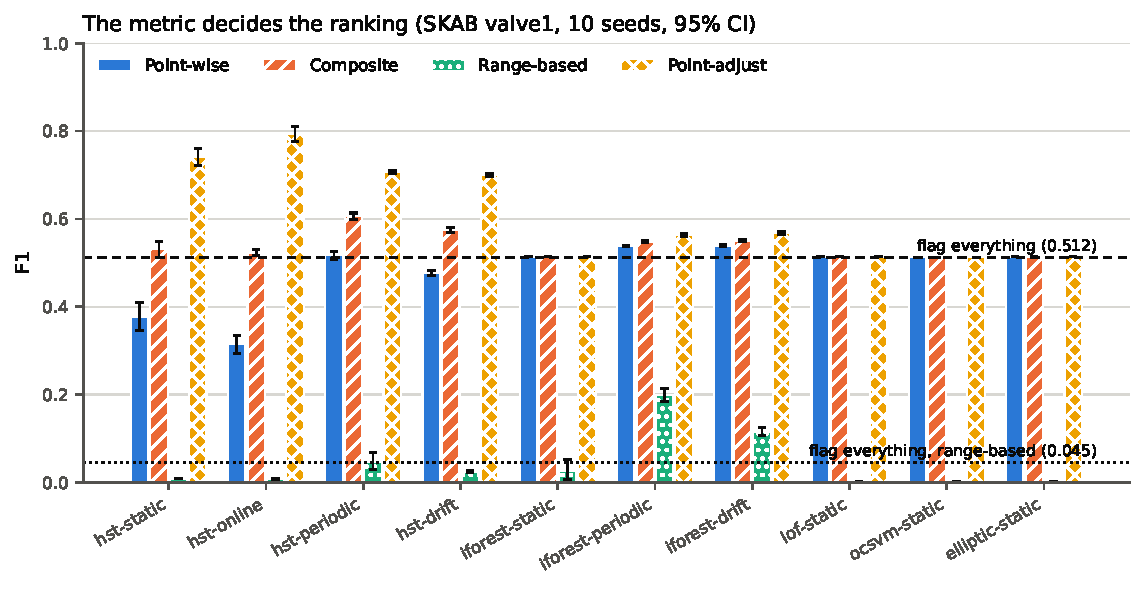
\includegraphics[width=\textwidth]{../results/figures/paper/metric_ranking.pdf}
\caption{The same runs under four scoring conventions, with 95\% bootstrap
intervals over \NSeeds{} seeds. The dashed line is the flag-everything
baseline.}
\label{fig:ranking}
\end{figure}

\begin{figure}[t]
\centering
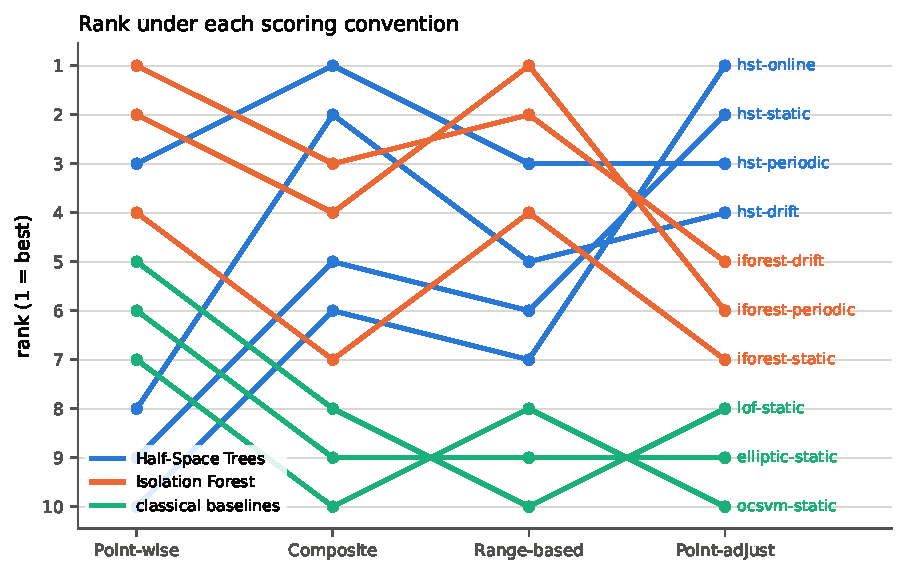
\includegraphics[width=0.72\textwidth]{../results/figures/paper/rank_flip.pdf}
\caption{Rank of each strategy under each convention. Colour is the model
family; each line is labelled with its strategy, and a line drawn faintly is one
whose rank is the same under all four conventions.}
\label{fig:rankflip}
\end{figure}

Point-adjust is included to show what it does to the table. We do not rely on it.
It credits an entire fault block for one flagged row, which on 390-row blocks
inflates every strategy at once. \citet{kim2022rigorous} showed that this lets
random predictions outscore trained models, and our test suite reproduces that
failure directly: two flags placed in a 300-row stream reach a point-adjust
recall of 1.0 against a point-wise recall of 0.01.

The last column of Table~\ref{tab:main} is the one to read first.
\NBeatPoint{} of \NStrategies{} strategies clear the flag-everything baseline
under point-wise scoring and \NBeatComposite{} clear it under the composite
score. A detector that flags 99\% of rows scores near the baseline by
construction, and several of the static baselines do exactly that.

Range-based scoring moves the baseline as well as the detectors, and it is
worth saying where it lands. Flagging every row produces one predicted range
spanning the stream, so its precision is divided by the number of true events
that range swallows, and the trivial baseline drops to \FlagAllRange{}.
Against that, \NBeatRange{} of \NStrategies{} strategies clear it. The
detectors are charged in the opposite direction: a permissive policy emits
thousands of short predicted ranges across each fault, and the cardinality
factor bills it for every fragment. Fragmentation is invisible to the other
three conventions and decisive under this one.

\subsection{Model against policy}
\label{sec:factorial}

The usual presentation of this comparison contrasts a static Isolation Forest
against an adaptive Half-Space Trees model, which confounds the two factors.
Figure~\ref{fig:factorial} crosses them.

\begin{figure}[t]
\centering
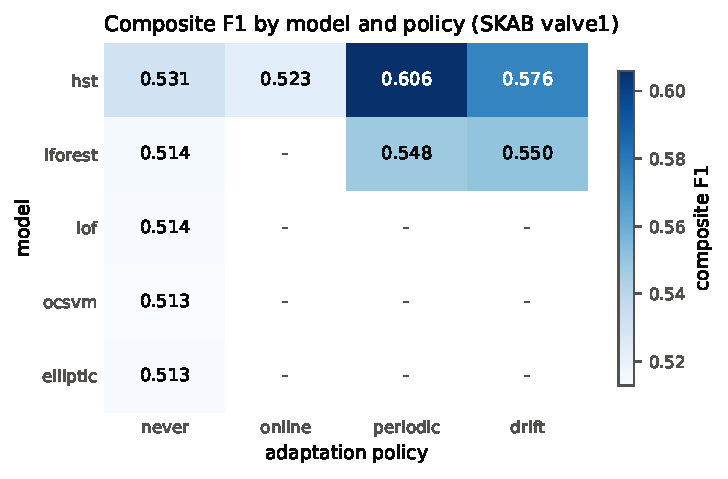
\includegraphics[width=0.62\textwidth]{../results/figures/paper/factorial.pdf}
\caption{Composite F1 by model and adaptation policy. The three classical
detectors appear only under \emph{never}: none supports an incremental update,
so for them adaptation could only mean a refit.}
\label{fig:factorial}
\end{figure}

Reading down a column separates the model from the policy, and reading across a
row separates the policy from the model. Both factors move the score, and the
policy moves it further: under the composite view the spread across policies
within Half-Space Trees is wider than the spread across models within the
\emph{never} column. The three classical baselines sit at the bottom of that
column together, all of them flagging over 99\% of rows, which is the same
failure the static Isolation Forest shows and not a quirk of one model.

The MCD estimator is worth a note, because it is the one baseline that had to
be nursed. It assumes the normal data forms one elliptical cloud, which SKAB's
multi-regime stream violates, and \texttt{scikit-learn} emits a determinant
warning on nearly every fit. On one NAB series it fails outright: 859 of the
1{,}000 warm-up rows there are exactly 0.0, so the robust support it selects is
entirely constant and the covariance is singular. We widen the support fraction
until it fits and record that we did. Both facts are reported because a
baseline that struggles for a stated structural reason is more useful than one
quietly dropped.

\subsection{Does the ranking survive the data?}
\label{sec:replication}

Seeds test whether a gap survives the randomness. They do not test whether it
survives a different recording, and on this data that is the harder question.
Figure~\ref{fig:segments} scores every strategy separately on each of the
\NRecordings{} source recordings that contain a fault.

\begin{figure}[t]
\centering
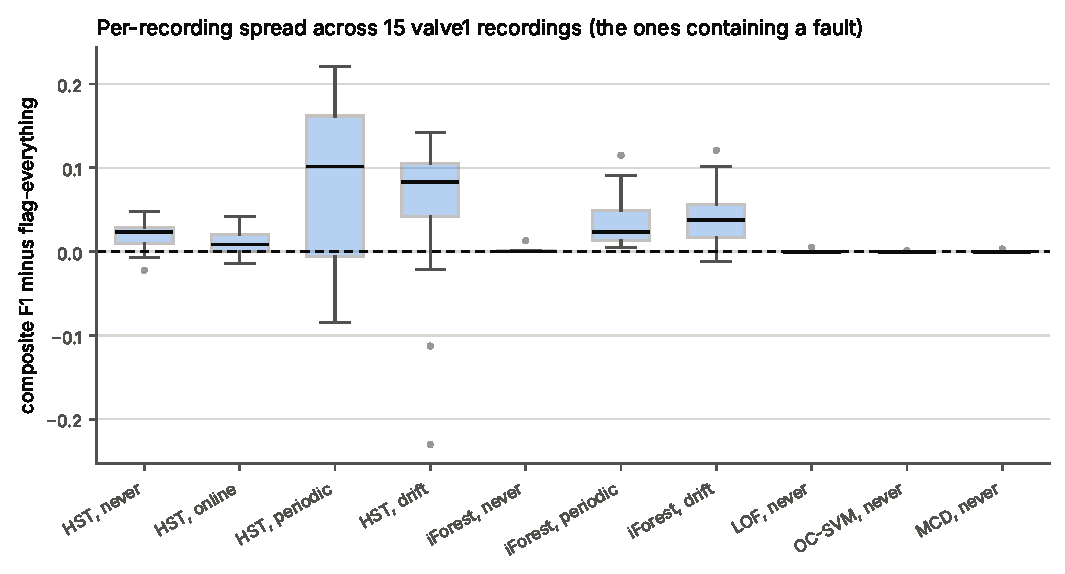
\includegraphics[width=\textwidth]{../results/figures/paper/segment_spread.pdf}
\caption{Composite F1 minus the flag-everything baseline, one point per source
recording, averaged over seeds. A box straddling zero is a strategy that does
not reliably beat flagging everything on an arbitrary recording.}
\label{fig:segments}
\end{figure}

Table~\ref{tab:significance} reports the paired comparisons the paper makes,
over both units. Of \NComparisons{} comparisons on the labelled stream,
\NSignificant{} survive Holm correction.

\begin{table}[t]
\centering
\small
\begin{tabular}{llcccc}
\toprule
Comparison & Metric & Unit & Mean diff. [95\% CI] & $p$ & Holm \\
\midrule
HST, periodic vs.\ HST, never & point & seed & $+0.140$ $[+0.109, +0.169]$ & 0.0020 & \yes \\
HST, drift vs.\ HST, never & point & seed & $+0.100$ $[+0.067, +0.131]$ & 0.0020 & \yes \\
HST, periodic vs.\ HST, drift & point & seed & $+0.040$ $[+0.035, +0.045]$ & 0.0020 & \yes \\
HST, periodic vs.\ HST, online & point & seed & $+0.203$ $[+0.184, +0.221]$ & 0.0020 & \yes \\
iForest, periodic vs.\ iForest, never & point & seed & $+0.024$ $[+0.023, +0.025]$ & 0.0020 & \yes \\
iForest, drift vs.\ iForest, never & point & seed & $+0.025$ $[+0.023, +0.026]$ & 0.0020 & \yes \\
HST, periodic vs.\ iForest, periodic & point & seed & $-0.021$ $[-0.029, -0.012]$ & 0.0059 & \yes \\
HST, never vs.\ iForest, never & point & seed & $-0.137$ $[-0.168, -0.104]$ & 0.0020 & \yes \\
HST, periodic vs.\ HST, never & point & segment & $+0.134$ $[+0.066, +0.198]$ & 0.0067 & \yes \\
HST, drift vs.\ HST, never & point & segment & $+0.085$ $[+0.016, +0.147]$ & 0.0353 & \no \\
HST, periodic vs.\ HST, drift & point & segment & $+0.049$ $[+0.004, +0.097]$ & 0.0554 & \no \\
HST, periodic vs.\ HST, online & point & segment & $+0.197$ $[+0.131, +0.260]$ & 0.0001 & \yes \\
iForest, periodic vs.\ iForest, never & point & segment & $+0.025$ $[+0.011, +0.041]$ & 0.0020 & \yes \\
iForest, drift vs.\ iForest, never & point & segment & $+0.026$ $[+0.008, +0.045]$ & 0.0151 & \no \\
HST, periodic vs.\ iForest, periodic & point & segment & $-0.029$ $[-0.086, +0.026]$ & 0.3894 & \no \\
HST, never vs.\ iForest, never & point & segment & $-0.138$ $[-0.146, -0.130]$ & 0.0001 & \yes \\
\midrule
HST, periodic vs.\ HST, never & composite & seed & $+0.075$ $[+0.058, +0.092]$ & 0.0020 & \yes \\
HST, drift vs.\ HST, never & composite & seed & $+0.045$ $[+0.027, +0.063]$ & 0.0020 & \yes \\
HST, periodic vs.\ HST, drift & composite & seed & $+0.030$ $[+0.026, +0.035]$ & 0.0020 & \yes \\
HST, periodic vs.\ HST, online & composite & seed & $+0.083$ $[+0.077, +0.089]$ & 0.0020 & \yes \\
iForest, periodic vs.\ iForest, never & composite & seed & $+0.033$ $[+0.032, +0.035]$ & 0.0020 & \yes \\
iForest, drift vs.\ iForest, never & composite & seed & $+0.036$ $[+0.034, +0.038]$ & 0.0020 & \yes \\
HST, periodic vs.\ iForest, periodic & composite & seed & $+0.058$ $[+0.052, +0.066]$ & 0.0020 & \yes \\
HST, never vs.\ iForest, never & composite & seed & $+0.017$ $[-0.002, +0.035]$ & 0.1934 & \no \\
HST, periodic vs.\ HST, never & composite & segment & $+0.064$ $[+0.010, +0.114]$ & 0.0479 & \no \\
HST, drift vs.\ HST, never & composite & segment & $+0.030$ $[-0.028, +0.078]$ & 0.1070 & \no \\
HST, periodic vs.\ HST, drift & composite & segment & $+0.034$ $[-0.016, +0.082]$ & 0.1876 & \no \\
HST, periodic vs.\ HST, online & composite & segment & $+0.072$ $[+0.021, +0.119]$ & 0.0256 & \no \\
iForest, periodic vs.\ iForest, never & composite & segment & $+0.036$ $[+0.021, +0.055]$ & 0.0002 & \yes \\
iForest, drift vs.\ iForest, never & composite & segment & $+0.038$ $[+0.021, +0.058]$ & 0.0006 & \yes \\
HST, periodic vs.\ iForest, periodic & composite & segment & $+0.045$ $[-0.003, +0.089]$ & 0.1070 & \no \\
HST, never vs.\ iForest, never & composite & segment & $+0.017$ $[+0.008, +0.025]$ & 0.0026 & \yes \\
\bottomrule
\end{tabular}

\caption{Paired comparisons on the labelled stream, over seeds and over source
recordings. Differences are the first strategy minus the second, with 95\%
bootstrap intervals. $p$ is a two-sided Wilcoxon signed-rank test; the last
column is the decision after Holm correction within the stream. Point-wise and
composite scoring are shown; the range-based comparisons are counted in the
totals quoted above and listed in full in \texttt{results/significance.csv}.}
\label{tab:significance}
\end{table}

The between-recording spread is the reason we consider the single-run tables
this project started with to have been unsupportable. It is wide enough that a
gap of a few hundredths, reported from one run, carries no information about
which policy to deploy.

It also complicates the aggregate ranking. \BestComposite{}, which wins
Table~\ref{tab:main} on the mean, fails to beat the trivial baseline on
\BestCompositeLosses{} of the \NRecordings{} recordings, and its interquartile
range in Figure~\ref{fig:segments} straddles zero. \SteadiestName{} scores
lower on average but fails on \SteadiestLosses{} of them, with an interquartile
range entirely above zero. Which of the two an operator should prefer depends on
whether they are averaging over many streams or deploying on one, and the mean
in the headline table cannot answer that.

\subsection{Drift detectors and detection timing}
\label{sec:timing}

The injected streams are where timing can be measured, because the change point
is known to the row and nothing in the stream is genuinely anomalous.
Table~\ref{tab:detectors} reports the delay at a 3\,sd shift.

\begin{table}[t]
\centering
\begin{tabular}{lccccc}
\toprule
Detector & sudden & incremental & gradual & recurring & False alarms / 1k \\
\midrule
\texttt{adwin} & 9 & 181 & 258 \ci{219}{296} & 20 & 1.92 \\
\texttt{adwin\_meanvar} & 9 & 181 & 104 \ci{85}{130} & 20 & 1.99 \\
\texttt{adwin\_var} & 9 & -- & 104 \ci{72}{130} & 30 & 0.29 \\
\texttt{kswin} & 107 \ci{59}{136} & 176 \ci{102}{242} & 202 \ci{90}{338} & 124 \ci{58}{194} & 2.77 \\
\texttt{pagehinkley} & 6 & 255 & 193 \ci{173}{212} & 5 & 1.53 \\
\bottomrule
\end{tabular}

\caption{Mean detection delay in rows at a 3\,sd shift, by drift shape, with 95\%
bootstrap intervals over seeds. A dash is a detector that never fired on that
shape. The last column is false alarms per 1{,}000 steps, averaged over shapes
and magnitudes.}
\label{tab:detectors}
\end{table}

\begin{figure}[t]
\centering
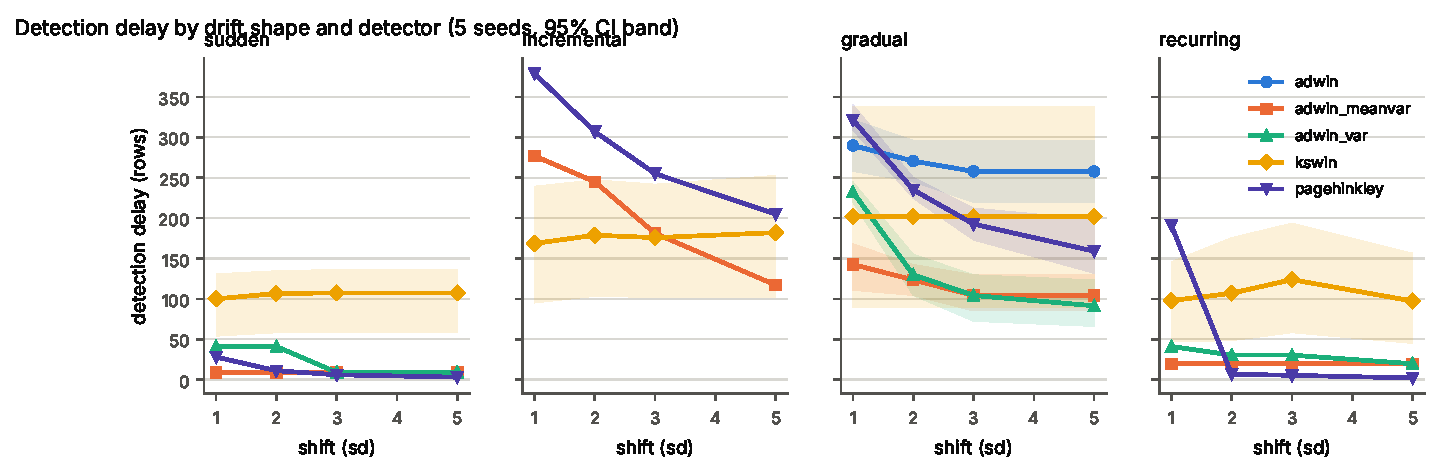
\includegraphics[width=\textwidth]{../results/figures/paper/detector_delay.pdf}
\caption{Detection delay against shift magnitude, one panel per drift shape.
Bands are 95\% bootstrap intervals over seeds.}
\label{fig:delay}
\end{figure}

Figure~\ref{fig:delay} plots the same measurement against magnitude. Two
shapes separate the detectors. A sudden step is caught quickly by anything that
watches the mean. Gradual drift, where the two regimes interleave before the
mean has moved, is the case a location detector cannot see: early in the
transition individual rows flip between the old and new regime, so the signal
grows spiky before its level changes. Feeding ADWIN the trailing \emph{variance}
of the monitored statistic, in place of its level, reacts to that. It cuts the
gradual delay by more than half, and it pays for that by going blind to a smooth
ramp, which shifts the mean without changing the spread: on the incremental
shape it never fires at all, at any magnitude. Running a mean ADWIN and a
variance ADWIN together and firing when either does recovers every shape and
keeps the better gradual delay.

Page-Hinkley was added to this comparison as a third opinion and turned out to
be the most interesting entry in the table. It is the quickest of the five on
both the sudden and the recurring shapes, and it raises fewer false alarms than
ADWIN while doing it. What it gives up is the incremental ramp, where it is the
slowest detector that fires at all: a cumulative sum needs the deviation to
accumulate, and a slow ramp supplies it slowly. That is a clean trade and not a
defect, and it is the kind of thing a single-detector study cannot see.
KSWIN is the one detector we would not recommend from these numbers: it is
slower than ADWIN on every shape and raises the most false alarms of the five.

The false-alarm column has to be read with Section~\ref{sec:limitations} in mind.
SKAB's anomaly-free recording is not stationary, so an unknown share of those
firings are the detector correctly noticing real process change.

\subsection{Transferring the calibration}
\label{sec:transfer}

Everything above is tuned on one industrial rig, which invites the objection
that the settings are fitted to it. Table~\ref{tab:transfer} applies the SKAB
threshold to \NNabSeries{} NAB series unchanged. NAB is univariate where SKAB
has eight sensors, and roughly 10\% anomalous where SKAB is \BaseRate\%, so it
breaks a transferred calibration in the ways that matter.

\begin{table}[t]
\centering
\small
\begin{tabular}{lccccc}
\toprule
NAB series & Best strategy & Flag-all & Point-wise F1 & Composite F1 & Beats \\
\midrule
ambient\_temperature & HST, periodic & 0.208 & 0.313 \ci{0.285}{0.338} & 0.543 \ci{0.463}{0.619} & \yes \\
cpu\_utilization\_asg & iForest, periodic & 0.162 & 0.338 \ci{0.317}{0.365} & 0.522 \ci{0.502}{0.546} & \yes \\
ec2\_request\_latency & HST, drift & 0.205 & 0.090 \ci{0.087}{0.093} & 0.376 \ci{0.363}{0.388} & \yes \\
machine\_temperature & MCD, never & 0.189 & 0.545 & 0.880 & \yes \\
nyc\_taxi & HST, online & 0.200 & 0.082 \ci{0.074}{0.093} & 0.388 \ci{0.327}{0.459} & \yes \\
rogue\_agent\_key\_updown & HST, drift & 0.219 & 0.040 \ci{0.040}{0.040} & 0.290 \ci{0.286}{0.294} & \yes \\
\bottomrule
\end{tabular}

\caption{NAB series with the SKAB threshold carried over unchanged, showing the
best strategy per series by composite F1. The flag-everything column is the
trivial baseline for that series.}
\label{tab:transfer}
\end{table}

\begin{figure}[t]
\centering
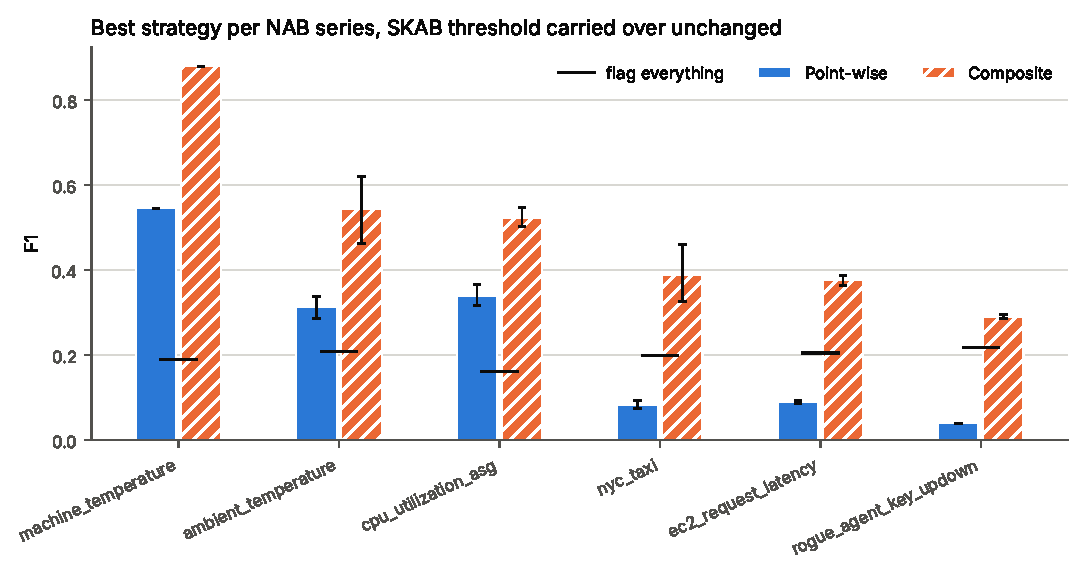
\includegraphics[width=\textwidth]{../results/figures/paper/transfer.pdf}
\caption{Best strategy per NAB series under point-wise and composite scoring,
with the trivial baseline marked.}
\label{fig:transfer}
\end{figure}

The metric effect reappears here and is larger than on SKAB
(Figure~\ref{fig:transfer}). Under point-wise
scoring the transferred setting beats the trivial baseline on
\NNabBeatsPoint{} of \NNabSeries{} series; under composite scoring it beats it
on \NNabBeatsComposite{}. NAB's anomalies are short and sparse, so point-wise
recall penalises a detector that flags a window without also flagging its
neighbourhood, which is the behaviour the composite score is built to credit.
The method carries across datasets in a way the point-wise numbers alone would
deny.

What does not carry is any particular strategy. \NNabDistinctWinners{}
different strategies take the top place across the \NNabSeries{} series, and
one of them is a classical static baseline. There is no ranking here to
transfer, only a method and a threshold that has to be set per deployment.

\subsection{Where event recall discriminates}
\label{sec:ucr}

Everything above is scored on data where the recall axis is nearly flat. On SKAB
every strategy catches every labelled event, so composite F1 is a ranking on
precision and nothing else. The UCR subset is here to supply the missing axis:
one anomaly per series, \NUcrSeries{} series, so a strategy either finds each
one or it does not.

\begin{table}[t]
\centering
\begin{tabular}{lccccc}
\toprule
Model, policy & Peak in window & Anomalies found & Composite F1 & Point-wise F1 & Alarm rate \\
\midrule
HST, never & 0.07 & 0.30 & 0.030 & 0.014 & 0.022 \\
HST, online & 0.06 & 0.42 & 0.023 & 0.013 & 0.032 \\
HST, periodic & 0.01 & 0.33 & 0.022 & 0.012 & 0.021 \\
HST, drift & 0.06 & 0.35 & 0.026 & 0.014 & 0.021 \\
iForest, never & 0.00 & 0.33 & 0.033 & 0.014 & 0.030 \\
iForest, periodic & 0.00 & 0.35 & 0.016 & 0.010 & 0.033 \\
iForest, drift & 0.01 & 0.26 & 0.019 & 0.011 & 0.029 \\
LOF, never & 0.12 & 0.50 & 0.030 & 0.021 & 0.046 \\
OC-SVM, never & 0.12 & 0.25 & 0.028 & 0.013 & 0.034 \\
MCD, never & 0.12 & 0.38 & 0.030 & 0.017 & 0.026 \\
\midrule
Flag everything & -- & 1.00 & 0.020 & 0.020 & 1.000 \\
\bottomrule
\end{tabular}

\caption{The UCR subset, averaged over \NUcrSeries{} series and \NSeeds{} seeds.
``Anomalies found'' is the proportion of series whose single anomaly the
strategy flagged at all, which is event-level recall when every series has
exactly one event. The trivial baseline finds every anomaly by definition and
pays for it in precision.}
\label{tab:ucr}
\end{table}

\begin{figure}[t]
\centering
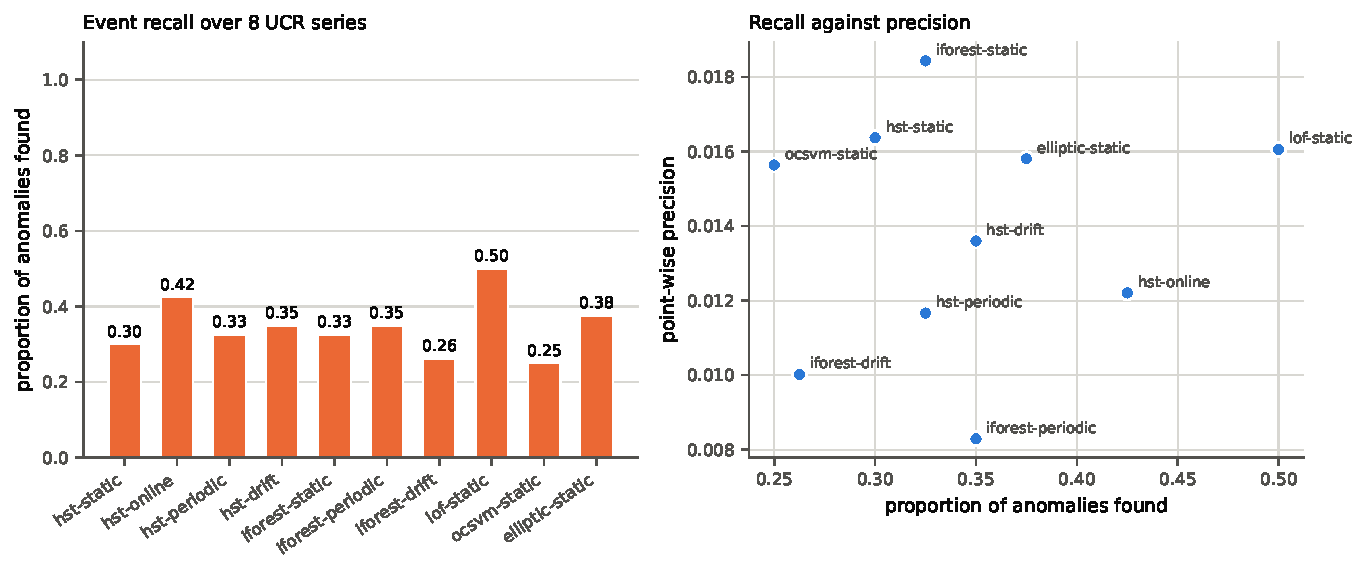
\includegraphics[width=\textwidth]{../results/figures/paper/ucr.pdf}
\caption{Left: the proportion of UCR anomalies each strategy found. Right: the
same quantity against point-wise precision, which is the trade the composite
score combines.}
\label{fig:ucr}
\end{figure}

The proportion of anomalies found (Figure~\ref{fig:ucr}) runs from
\WorstUcrFound{} for \WorstUcrName{} to \BestUcrFound{} for \BestUcrName{}, a
spread of \UcrRecallSpread{}. That spread is the first thing to note. It is a real
difference between strategies that SKAB cannot show at all and NAB shows only
partially, and it exists because the benchmark was built so a detector can miss.

The second thing to note is the level. The best strategy here finds
\BestUcrFound{} of the anomalies. Not one of the ten finds most of them, and
that is on a subset chosen for being short and tractable. Whatever these
policies are doing on SKAB, they are not solving this.

The base rate is \UcrBaseRate\%, which puts the trivial baseline at
\UcrFlagAll{} rather than the \FlagAll{} it reaches on SKAB. That is a much
lower bar and it is the bar a detector should face: where anomalies are genuinely
rare, flagging everything is obviously useless, and a benchmark on which it looks
competitive is the problem \citet{wu2023flawed} were describing.
\NUcrBeatComposite{} of \NStrategies{} strategies clear it under the composite
score and \NUcrBeatPoint{} point-wise, but the margins are small enough that
clearing it is not much of a claim.

\paragraph{The archive's own criterion.} Scoring UCR with a thresholded F1 is
not what its authors intended. They score a series as solved when the single
highest anomaly score falls inside the labelled window, and they argue for that
because it needs no threshold, so the cutoff stops being part of what is
measured. Substituting our own convention for theirs would be the exact move
this paper criticises, so Table~\ref{tab:ucr} reports both. Under the archive's
criterion the best strategy is \BestUcrTopOne{} at \BestUcrTopOneVal{}, the
worst manages \WorstUcrTopOneVal{}, and the average across all ten is
\MeanUcrTopOne{}. The two protocols do not even agree on a winner
(\TopOneAgreesWithComposite{}), which is the same disagreement this paper
documents between conventions, now reproduced between our scoring and the
dataset author's.

\paragraph{Adaptation does not help here.} The best composite score on this data
belongs to \BestUcrComposite{}, and the most anomalies are found by
\BestUcrName{}. Both are configured to \emph{\BestUcrPolicy{}}, and neither is
one of the \NUcrAdaptive{} adaptive configurations. On the benchmark built to be hard,
the question this paper is about stops mattering: the policies are separated by
less than the noise, and the classical static detectors are as good as anything
with a rebuild schedule. We report that because it is what the data says, and
because a paper that found adaptation mattered on two datasets and quietly left
out the third would be doing what its own introduction complains about.

\subsection{Sensitivity to the constants we chose}
\label{sec:ablation}

Three values in this design were picked by judgement: the warm-up length of
1{,}000 rows, the 750-step horizon within which a detection is credited to a
change point, and the 250-step cooldown after a detector fires.
Figure~\ref{fig:ablation} varies the first two.

\begin{figure}[t]
\centering
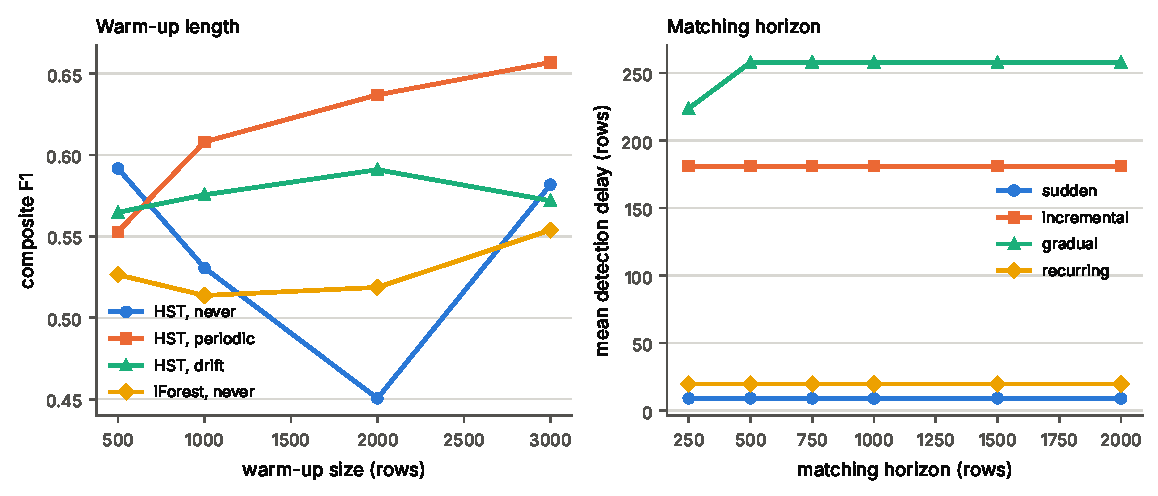
\includegraphics[width=\textwidth]{../results/figures/paper/ablation.pdf}
\caption{Left: composite F1 against warm-up length. Right: mean detection delay
against the matching horizon. Changing the warm-up also changes which rows are
scored, so the base rate moves with it; the raw counts are in
\texttt{results/ablation\_warmup.csv}.}
\label{fig:ablation}
\end{figure}

The matching horizon turns out not to be load-bearing. Past 500 steps the
mean delay is identical for every drift shape, and the gradual case is the
only one that moves at all between the shortest setting and the default. A
detection either lands close to the change point or does not land at all, so
the exact cut-off has little to decide.

Warm-up length is the constant that does matter, and it does not treat the
policies alike: the periodic schedule improves steadily as the warm-up
lengthens, while the drift-triggered one is flat and the static baseline moves
erratically. We report this as a sensitivity and not as a tuning result,
because changing the warm-up also changes which rows are scored, and on a
stream with unevenly spaced faults that moves the base rate underneath the
comparison. The per-setting base rates are in
\texttt{results/ablation\_warmup.csv}.

The cooldown behaves as it was designed to and buys less than expected. At the
two shortest settings the number of rebuilds is identical, which says the
detector's own firing spacing already exceeds them; only at the longest
setting does suppression bite hard enough to halve the rebuilds. None of the
conclusions above depends on the value we picked.

\subsection{Cost}
\label{sec:cost}

A streaming method that cannot keep up with the stream is not one.
Table~\ref{tab:cost} reports throughput on a single laptop core.

\begin{table}[t]
\centering
\begin{tabular}{lcc}
\toprule
Model, policy & Rows / second & Rebuilds \\
\midrule
HST, never & 19,325 & 0.0 \\
HST, online & 10,324 & 0.0 \\
HST, periodic & 2,530 & 17.0 \\
HST, drift & 947 & 35.0 \\
iForest, never & 29,714 & 0.0 \\
iForest, periodic & 2,430 & 17.0 \\
iForest, drift & 844 & 35.0 \\
LOF, never & 38,085 & 0.0 \\
OC-SVM, never & 129,212 & 0.0 \\
MCD, never & 34,839 & 0.0 \\
\bottomrule
\end{tabular}

\caption{Throughput and rebuild count on the labelled stream, averaged over
seeds. The static sklearn baselines score in vectorised blocks; the Half-Space
Trees implementation scores one observation at a time, which is the honest cost
of an online model in this library.}
\label{tab:cost}
\end{table}

The spread here is a property of the implementations, not of the algorithms:
Half-Space Trees is scored one observation at a time in \texttt{river}, while
the sklearn baselines are scored in vectorised blocks. It is reported because a
comparison that leaves cost out is incomplete. On this hardware the slowest
strategy, \SlowestModel{}, processes \SlowestRows{} rows per second against
\FastestRows{} for \FastestModel{}, a factor of about \SpeedRatio{}. Every
strategy here keeps up with anything a single sensor rig produces; the figure
starts to matter when one detector is run across thousands of streams at once.


\section{Discussion}

\subsection{What a practitioner should take from this}

The first decision in an evaluation is which convention to score under, and on
this data that decision moves the answer more than the choice of adaptation
policy does. It should therefore be made deliberately and stated. Inheriting it
from whichever paper the code was adapted from is how it usually happens.

The convention follows from what an alarm costs. If an operator investigates
each alarm individually, every false row is paid for and point-wise precision is
the quantity that matters. If an operator investigates each \emph{episode}, a
detector that flags one row of a fault has done its job and the composite or
range-based view describes the deployment better. These are different questions
about the same predictions. Reporting one number without saying which question
it answers leaves the reader to guess.

The second suggestion is procedural. Quote a trivial baseline next to every
score. At a base rate of \BaseRate\%, flagging every row scores \FlagAll{} under
point-wise F1, which is higher than several published-looking numbers. We spent
part of this project rediscovering that a detector can clear 0.5 F1 while doing
nothing at all, and the baseline column is what stops that from happening
quietly.

The third point is about which number to read once both of those are settled.
The strategy that wins our headline table on the mean is not the one we would
deploy. \BestComposite{} takes the top place on average and still fails to beat
the trivial baseline on \BestCompositeLosses{} of the \NRecordings{} individual
recordings, with an interquartile range that straddles zero;
\SteadiestName{} scores lower on average and fails on \SteadiestLosses{}. A mean
over streams answers a question about a benchmark. An operator with one stream
is asking a different question, and the spread across recordings is what answers
it.

\subsection{On the adaptation question itself}

Stripped of the metric problem, the practical picture is narrower than
``adaptive detection works better''. Rebuilding on a schedule and rebuilding on
detected change both beat leaving the model alone, and the margin between the
two is small next to the margin between either of them and the trivial
baseline. The case for drift-triggered rebuilding is not that it scores higher.
It is that it reacts to evidence and not to a clock, which lets it notice a
sudden shift within a few rows instead of waiting for the next scheduled
rebuild, and keeps it from rebuilding on a stream that has not moved.

That argument is about the shape of the response, and Section~\ref{sec:timing}
is where it is measured. It is a smaller claim than the one we expected to make
when the project started.

\subsection{Limitations}
\label{sec:limitations}

These are constraints on what the numbers above can support, and several of them
cut against our own results.

\paragraph{The base recording is not stationary.} SKAB's anomaly-free recording
has no annotated faults but the process drifts on its own. Running with no
injected drift still produces adaptations, at nearly the same positions as with a
3\,sd step injected. False-alarm counts on the injected streams are therefore an
upper bound and not a measurement: some of those firings are the detector
correctly noticing real process change for which we have no ground truth. For
the same reason we do not report detection \emph{rate}, which comes out at 1.0
for every magnitude including the zero control, because a firing always lands
within the matching horizon of an arbitrary point.

\paragraph{The labelled stream is concatenated.} The individual \texttt{valve1}
recordings are about 1{,}000 rows, too short to warm up on and still leave stream
to measure, so we join 16 of them. The joins are genuine regime
changes of unknown magnitude. That is why this stream is used for anomaly
quality only and never for drift timing, and it is why we also report per
recording, where the joins are not inside the scored region.

\paragraph{Event recall saturates on SKAB.} SKAB's faults are long, so on the
labelled stream every strategy catches every event and event-level recall is 1.0
across the board. Composite F1 there reduces to a precision-driven ranking. That
is the correct operational picture, and it is what point-wise scoring obscured,
but the recall axis carries no information on that particular stream. This is
why the UCR subset is in the paper, and Section~\ref{sec:ucr} is where the
recall axis does some work. The limitation is not removed so much as bounded: it
applies to SKAB, partly to NAB, and not to UCR.

\paragraph{Three datasets, one of them contested.} \citet{wu2023flawed} argue
that NAB and benchmarks like it are flawed enough to mislead. We use NAB only to
ask whether a calibration transfers, which is a weaker use than ranking
detectors on it, but the criticism still applies to Section~\ref{sec:transfer}.
The UCR archive is those authors' own replacement and we use a subset of it, so
the study is no longer resting on the benchmarks they criticised. It is a
subset, though: \NUcrSeries{} of 250, chosen by a stated rule and bounded by
what one core can run. A study with the compute to take all 250 would be a
stronger test than ours.

\paragraph{No deep or model-pooling baselines.} The comparison covers one online
model, one static ensemble and three classical detectors. It does not include the
autoencoder and model-pooling systems that dominate recent leaderboards
\citep{yoon2022arcus}. Our claim is about how adaptation policies compare under
different scoring conventions, not about the state of the art in raw detection
quality, and the metric result is if anything more consequential for those
systems, since they are usually reported under point-adjust.

\paragraph{The threshold is a deployment choice.} It has to be set from the
expected anomaly rate of the specific stream. We measured what carrying one
setting across datasets costs instead of assuming it away, but no rule here
removes the need to choose.

\paragraph{One machine, one implementation.} Throughput in
Section~\ref{sec:cost} is from a single laptop core and a specific pair of
libraries. It supports statements about relative cost between the strategies and
not about absolute deployability.

\subsection{Reproducing this}

Every number in this paper, including the ones in the prose, is generated from
the committed CSV files by \texttt{scripts/make\_paper\_tables.py}; the
manuscript contains no hand-typed values. The experiments regenerate with

\begin{quote}
\texttt{python scripts/run\_multiseed.py}\\
\texttt{python scripts/run\_sweep.py -{}-seeds 5}\\
\texttt{python scripts/run\_ablation.py}\\
\texttt{python scripts/run\_throughput.py}\\
\texttt{python scripts/make\_paper\_figures.py}\\
\texttt{python scripts/make\_paper\_tables.py}
\end{quote}

Timing gets its own short run because it is the one measurement sensitive to
what else the machine is doing, and the grid occupies a core for the better part
of an hour.

The full grid takes under an hour on one core. The test suite covers the metric
implementations against hand-computed values, the statistics against constructed
data with known answers, and the fast scoring path against the plain one.

\section{Conclusion}

We compared four adaptation policies for a streaming anomaly detector, crossed
with the model they run on, repeated over \NSeeds{} seeds and \NRecordings{}
recordings, and scored the same runs under four published conventions. The four
conventions produce \NDistinctWinners{} different winners.

The narrow finding is about one benchmark and one family of detectors. The
general one is that a paper reporting a single scoring convention has not
established which policy is better, only which policy that convention prefers.
On the stream studied here, \MoverName{} moves from \MoverPointRank{} to
\MoverCompositeRank{} of \NStrategies{} on identical predictions.

The third dataset put a limit on all of it. On the UCR subset no policy
separates from the others, the classical static detectors match anything with a
rebuild schedule, and under the archive's own criterion the field as a whole
puts its peak score inside the labelled window on \MeanUcrTopOne{} of series.
The comparison this paper is built around is worth making on SKAB and is close
to meaningless on the benchmark built to be hard. We would rather finish on that
than on the part that worked.


\bibliography{references}

\end{document}
